\documentclass[10pt, conference]{IEEEtran}
% \IEEEoverridecommandlockouts
% The preceding line is only needed to identify funding in the first footnote. If that is unneeded, please comment it out.
\usepackage{cite}
\usepackage{hyperref}
\usepackage{amsmath,amssymb,amsfonts}
\usepackage{algorithmic}
\usepackage{graphicx}
\usepackage{textcomp}
\usepackage{xcolor}
\usepackage{orcidlink}
\usepackage{acronym}
\def\BibTeX{{\rm B\kern-.05em{\sc i\kern-.025em b}\kern-.08em
    T\kern-.1667em\lower.7ex\hbox{E}\kern-.125emX}}



%---- PACKAGES
%\usepackage{todonotes}
\usepackage{amssymb}
\usepackage{hyperref}
\usepackage[plain]{fancyref}
\usepackage{ifdraft}
%\usepackage{subcaption}
\let\labelindent\relax
\usepackage[inline]{enumitem}
\usepackage{xcolor}
\usepackage{xspace}
\usepackage[final]{listings}
\usepackage{acronym}
\usepackage{url}
\usepackage{amsmath}
\usepackage{amssymb}
\usepackage{booktabs} % For formal tables
\usepackage{subfig}
\usepackage{balance}
\usepackage{dirtree}


\usepackage[ruled]{algorithm2e} % For algorithms
\renewcommand{\algorithmcfname}{ALGORITHM}
\newcommand{\subparagraph}{}


\usepackage{etoolbox}
\makeatletter
\patchcmd{\@makecaption}
  {\scshape}
  {}
  {}
  {}
\patchcmd{\@makecaption}
  {\\}
  {.\ }
  {}
  {}
\makeatother

%\let\refsection\relax
%\usepackage
%  [backend=bibtex,
%  style=ieee,
%   maxnames=5,
%   firstinits=true,
%   hyperref=true,
%   natbib=true,
%   url=false,
%   doi=false]{biblatex}



%
%----[ Biber ]----
%\addbibresource[datatype=bibtex]{local.bib}
%\addbibresource[datatype=bibtex]{bib/tools.bib}
%\addbibresource[datatype=bibtex]{bib/compsci.bib}
%\addbibresource[datatype=bibtex]{bib/learning.bib}
%\nocite{*}
%
%\newbibmacro{name:newformat}{%
%    \printnames{authors}
%%   \textbf{\namepartfamily}  % #1->\namepartfamily, #2->\namepartfamilyi
%%   \textbf{\namepartgiven}   % #3->\namepartgiven,  #4->\namepartgiveni
%%   [prefix: \namepartprefix] % #5->\namepartprefix, #6->\namepartprefixi
%%   [suffix: \namepartsuffix] % #7->\namepartsuffix, #8->\namepartsuffixi
%}
%
%\DeclareNameFormat{newformat}{%
%  \usebibmacro{name:newformat}{\textbf{#1}}{\textbf{#3}}{#5}{#7}%
%  \usebibmacro{name:andothers}%
%%  \nameparts{#1}% split the name data, will not be necessary in future versions
%%  \usebibmacro{name:newformat}%
%%  \usebibmacro{name:andothers}%
%}
%

%\AtEveryBibitem
%{
%   \clearlist{address}
%   \clearfield{date}
%   \clearfield{doi}
%   \clearfield{eprint}
%   \clearfield{isbn}
%   \clearfield{issn}
%   \clearfield{month}
%   \clearfield{note}
%%   \clearfield{pages}
%   \clearlist{location}
%%   \clearfield{series}
%   \clearfield{url}
%   \clearname{editor}
%   \ifentrytype{inproceedings}
%     {\clearfield{day}
%      \clearfield{month}
%      \clearfield{volume}}{}
%}
%
%\DeclareFieldFormat*{title}{\textsl{#1}\isdot}
%\DeclareFieldFormat*{journaltitle}{#1}
%\DeclareFieldFormat*{booktitle}{#1}
%
%\renewbibmacro{in:}{} % supress 'In: ' form
%
%\DeclareSourcemap
% {\maps[datatype=bibtex,overwrite]
%   {% Tag entries (through keywords)
%    \map
%      {\step[fieldsource=booktitle,
%       match=\regexp{[Pp]roceedings}, replace={Proc.}]}
%        \map
%      {\step[fieldsource=booktitle,
%       match=\regexp{[Ii]nternational\s+[Cc]onference}, replace={Intl. Conf.}]}
%    \map
%      {\step[fieldsource=journal,
%       match=\regexp{[Jj]ournal}, replace={Jour.}]}
%    \map
%      {\step[fieldsource=journal,
%       match=\regexp{[Tt]ransactions}, replace={Trans.}]}
%    \map
%      {\step[fieldsource=booktitle,
%       match=\regexp{[Pp]roceedings\s+of\s+the.+[Ee]uropean\s+[Cc]onference\s+in}, replace={European Conf. in}]}
%    \map
%      {\step[fieldsource=booktitle,
%       match=\regexp{In\s+[Pp]roceedings\s+of\s+the.+[Ss]ymposium\s+on}, replace={Symp. on}]}
%    \map
%      {\step[fieldsource=booktitle,
%       match=\regexp{[Pp]roceedings\s+of\s+the.+[Ii]nternational\s+[Cc]onference\s+on}, replace={Intl. Conf. on}]}
%    \map
%      {\step[fieldsource=booktitle,
%       match=\regexp{[Pp]roceedings\s+of\s+the.+[Ii]nternational\s+[Ww]orkshop\s+on}, replace={Intl. Workshop on}]}}}
%

%color
\definecolor{OliveGreen}{rgb}{0,0.6,0.3}

%References
%% Listings
\def\fref{\Fref} % treat all \frefs as \Frefs
\renewcommand{\lstlistingname}{Snippet}
\newcommand*{\fancyreflstlabelprefix}{lst}
\newcommand*{\Freflstname}{\lstlistingname}
\newcommand*{\freflstname}{\MakeLowercase{\lstlistingname}}
\Frefformat{vario}{\fancyreflstlabelprefix}%
  {\Freflstname\fancyrefdefaultspacing#1#3}
\frefformat{vario}{\fancyreflstlabelprefix}%
  {\freflstname\fancyrefdefaultspacing#1#3}
\Frefformat{plain}{\fancyreflstlabelprefix}%
  {\Freflstname\fancyrefdefaultspacing#1}
\frefformat{plain}{\fancyreflstlabelprefix}%
  {\freflstname\fancyrefdefaultspacing#1}

\renewcommand{\tablename}{Table}  
  
% ln delimiter
\newcommand*{\fancyreflnlabelprefix}{ln}
\newcommand*{\Freflnname}{Line}
\newcommand*{\freflnname}{\MakeLowercase{\Freflnname}}
\Frefformat{vario}{\fancyreflnlabelprefix}%
  {\Freflnname\fancyrefdefaultspacing#1#3}
\frefformat{vario}{\fancyreflnlabelprefix}%
  {\freflnname\fancyrefdefaultspacing#1#3}
\Frefformat{plain}{\fancyreflnlabelprefix}%
  {\Freflnname\fancyrefdefaultspacing#1}
\frefformat{plain}{\fancyreflnlabelprefix}%
  {\freflnname\fancyrefdefaultspacing#1}    


%JavaScript definition
\lstdefinelanguage{JavaScript}{
keywords={typeof, new, true, false, catch, function, return, null, catch, switch, var, if, in, for, while, do, else, case, break, throw, this, instanceof},
keywordstyle=\color{purple}\bfseries,
ndkeywords={},
ndkeywordstyle=\color{blue}\bfseries,
identifierstyle=\color{black},
sensitive=false,
comment=[l]{//},
morecomment=[s]{/*}{*/},
commentstyle=\color{OliveGreen}\ttfamily,
stringstyle=\color{OliveGreen}\ttfamily,
morestring=[b]',
morestring=[b]"
}
\usepackage{color}
\definecolor{gray97}{gray}{.97}
\definecolor{gray90}{gray}{.90}
\definecolor{gray75}{gray}{.75}
\definecolor{gray45}{gray}{.45}
\definecolor{codegreen}{rgb}{0,0.6,0}
\definecolor{codered}{rgb}{0.6,0,0}
\definecolor{codegray}{rgb}{0.5,0.5,0.5}
\definecolor{codepurple}{rgb}{0.58,0,0.82}
\lstset{ frame=single,
	framerule=0.2pt,
	framextopmargin=3pt,
	framexbottommargin=3pt,
	framexleftmargin=0.4cm,
	framesep=0.5pt,
	rulesep=0.5pt,
	backgroundcolor=\color{gray97},
	rulesepcolor=\color{black},
	xleftmargin=0.7cm,
	%
	stringstyle=\ttfamily,
	showstringspaces = false,
	basicstyle=\fontsize{6pt}{7pt}\ttfamily,
	keywordstyle=\color{magenta}\bfseries,
	numberstyle=\tiny\color{codegray},
	stringstyle=\color{codepurple},
	commentstyle=\color{codegreen},
	%
	numbers=left,
	numbersep=15pt,
	numberstyle=\tiny,
	numberfirstline = false,
	breaklines=true,
	escapeinside={(*@}{@*)},
	literate={~} {$\sim$}{1}
}

\lstdefinestyle{floating}{%
  frame=none,
  float=htb,
  captionpos=b
}

% context traits listings
\lstdefinestyle{ctxtraits}
 {language=JavaScript,
  frame=lines,
  showstringspaces=false,
  keywordstyle=\tt\bf,
  tabsize=3,
  style=floating,
  morekeywords={Trait, cop, Context, activate, deactivate, adapt, addObjectPolicy, manager}
}

%context traits environment    
\lstnewenvironment{ctxtraits}[1][]
 {\lstset{style=ctxtraits,#1}}{}  


 % Context Traits in line source code
\newcommand{\scode}[1]{\textrm{\texttt{#1}}}
\def\scode{\lstinline[style=ctxtraits]}

%----[ Commands ]---
%Latins
\newcommand{\eg}{\emph{e.g.,}\xspace}
\newcommand{\ie}{\emph{i.e.,}\xspace}
\newcommand{\etal}{\emph{et al.}\xspace}
\newcommand{\aka}{\emph{a.k.a.,}\xspace}
\newcommand{\cf}{\emph{cf.}\xspace}
\newcommand{\mref}{\textcolor{red}{[REF]}\xspace}
\newcommand{\secref}[1]{Section~\ref{#1}\xspace}
\newcommand{\figref}[1]{Fig.~\ref{#1}\xspace}
\newcommand{\listref}[1]{Listing~\ref{#1}\xspace}
\newcommand{\tabref}[1]{Table~\ref{#1}\xspace}

\newcommand{\itdroid}{\textsc{itDroid}\xspace}
\newcommand{\numapps}{\textcolor{red}{80}\xspace}


\newcommand{\ctx}[1]{\texttt{\textsc{#1}}}


%comments
% xcolor
\definecolor{author}{rgb}{.5, .5, .5}
\definecolor{comment}{rgb}{.1, .0, .9}
\definecolor{note}{rgb}{.9, .4, .0}
\definecolor{idea}{rgb}{.1, .7, .0}
\definecolor{missing}{rgb}{.9, .1, .0}
\definecolor{deleteme}{rgb}{.9, .1, .0}

\newcommand{\MARIO}[2][comment]{\authorcomment[#1]{MLV}{#2}}
\newcommand{\CAMILO}[2][comment]{\authorcomment[#1]{CEV}{#2}}
\newcommand{\ALEJO}[2][comment]{\authorcomment[#1]{AMR}{#2}}
\newcommand{\ANA}[2][comment]{\authorcomment[#1]{AMH}{#2}}
\newcommand{\MICHAEL}[2][comment]{\authorcomment[#1]{MOR}{#2}}
\newcommand{\LAURA}[2][comment]{\authorcomment[#1]{LBJ}{#2}}

\newcommand{\authorcomment}[3][comment]
  {\noindent
      \fbox{\footnotesize\textcolor{author}{\textsc{#2}}}
      \textcolor{#1}{\textsl{#3}}{}}




% !TEX root = main.tex

% \acrodef{APK}{Android Application Package}
% \acrodef{AI}{Artificial Intelligence}
% \acrodef{WCAG}{Web Content Accessibility Guidelines}
% \acrodef{UI}{User Interface}
% \acrodef{AOM}{Accessibility Object Model}
% % \acrodef{a11y}{Accessibility}

\acrodef{VR}{virtual reality}
\acrodef{NLP}{natural language processing}
\acrodef{HCI}{human-computer interaction}
\acrodef{AAC}{augmentative and alternative communication}
\begin{document}

\title{EyeNav: Accessible Webpage Interaction and Testing using Eye-tracking and NLP}

\author{
    \IEEEauthorblockN{
        Juan Diego Yepes-Parra \orcidlink{0009-0007-0672-1473}, 
        Camilo Escobar-Velásquez \orcidlink{0000-0001-8414-9301}
    }
    \IEEEauthorblockA{
        \textit{Universidad de los Andes, Colombia} \\
        \{j.yepes, ca.escobar2434\}@uniandes.edu.co
    }
}

\maketitle

\begin{abstract}
In the field of \ac{HCI}, alternative interaction methods are becoming increasingly popular and commercialy available. From this opportunity came EyeNav, a system that combines eye-tracking and natural language processing (NLP) to enhance accessibility and enable automated test generation. The integration of these technologies for intuitive web interaction, using pointer control via gaze and natural language processing for interpreting user intentions, also presents a record-and-replay module for generating automated test scripts. Envisioned for users with motor disabilities, developers, usability testers, and general users interested in exploring novel multimodal web interactions.
The ultimate goal is to demonstrate that this tool can be used not only as a possible assistive technology but also as an innovative approach to software testing. The tool is available publicly at \href{https://thesoftwaredesignlab.github.io/EyeNav/}{https://thesoftwaredesignlab.github.io/EyeNav/}, accompanied with a demonstration video \href{https://thesoftwaredesignlab.github.io/EyeNav/video.html}{https://thesoftwaredesignlab.github.io/EyeNav/video.html} 
\end{abstract}


\begin{IEEEkeywords}
Eye-tracking; Automated Test Generation; Assistive Technology; Natural Language Processing; Web Applications; Accessibility.
\end{IEEEkeywords}

% !TEX root = main.tex

\section{Introduction}

Alternative interaction methods are becoming increasingly prevalent across modern computing systems. 
Devices such as smartphones and tablets~\cite{apple2024accessibility, honor_magic6pro_specs}, wearables\cite{tobii_glasses_x}, and headsets\cite{apple_vision_pro_2025,playstation_vr2_specs,vive_pro2_2025} frequently incorporate novel input technologies, enabling more natural, inclusive, and adaptive user experiences~\cite{dondi2023gazehci, fernandes2023eyevr}.
These emerging methods hold particular significance for accessibility applications, as they provide alternative means for users with motor impairments or other physical limitations to interact with digital content~\cite{hsieh2024increasing}.

Although eye-tracking has been the subject of research for many years\cite{gips1996eagleeyes}, it is increasingly emerging as an input modality through its growing integration into everyday consumer devices. When implemented effectively, it enables precise, intuitive, and hands-free control~\cite{huang2024visionpro}.

On the contrary, \ac{NLP} is already well establised as a compelling input method, enabling users to interact with software through spoken commands. 
From voice-enabled code generation~\cite{serenade2025} to smart assistants, speech interfaces are widely researched and deployed. Still, these systems can become frustrating if user intent is misinterpreted or ignored, highlighting the importance of robust semantic parsing and contextual understanding~\cite{mozafari2020chatbot, liu2024chatgpt}. 

EyeNav is a tool developed to introduce a novel input method, integrating real-time eye-tracking with natural language interaction within web applications. This system facilitates interactions that are intuitive, accessible, and innovative.

Implemented as a Chrome extension, EyeNav allows users to interact with pages via gaze-based control and spoken commands. It also integrates a record-and-replay module to support automated testing workflows using the Gherkin standart.

Initially designed for users with motor impairments; it also holds potential for developers interested in hands-free browser control or rapid prototyping, usability professionals conducting accessibility evaluations in web environments, and general users exploring novel multimodal web interactions. By bridging assistive technologies and test automation, the prototype facilitates broader evaluation and integration of accessibility focused solutions within mainstream web contexts.

This paper outlines our approach overview, methodology, evaluation and discusses implementation and future work considerations for the system.

% !TEX root = main.tex

\section{Related Work}

\subsection{Eye-tracking in HCI}

The use of eye-tracking has been extensively researched and applied across a wide range of domains. Although initially conceived primarily for behavioral and psychological studies, a practice that remains prevalent, eye-tracking was originally employed to gain insights into human cognition and behavior, rather than as a mechanism for user input. For instance, Zelinskyi et al.\ developed a Chrome extension designed to collect eye-tracking data for behavioral analysis~\cite{zelinskyi2024eyetracking}. Similarly, Jacob and Karn discuss the role of eye-tracking in usability research, emphasizing its value for evaluating user interfaces~\cite{jacob2003commentary}.

Over time, researchers have explored eye-tracking as a viable input modality within HCI. Notably, Gips et al.\ introduced an eye-controlled system in the late 1990s, specifically aimed at improving accessibility for individuals with motor impairments~\cite{gips1996eagleeyes}. Such efforts have continued into recent years and different applications. Dondi et al.\ examined the role of eye-tracking in immersive museum and exhibition experiences~\cite{dondi2023gazehci}, while Karlander and Wang integrated eye-tracking into artificial intelligence image editing software~\cite{karlander2023ai}.

Recent advancements in consumer-grade augmented and virtual reality headsets, such as the Meta Quest Pro, Pico 4 Pro, and Apple Vision Pro, have significantly increased the adoption of integrated eye-tracking technologies~\cite{huang2024visionpro}. Some of these devices, most notably the Apple Vision Pro, rely entirely on eye-tracking and hand gestures for user interaction, eliminating the need for traditional physical input peripherals.

Accessible HCI has also integrated eye-tracking. For example, Wang et al.\ introduced \textit{GazePrompt}, a gaze-aware reading aid for low-vision users. The system offers line-switching support, which highlights or indicates the next line as the user reads, and difficult-word support, which automatically magnifies or reads aloud a word when user hesitation is detected~\cite{wang2024gazeprompt}. Additionally, commercial eye-tracking hardware is increasingly embedded in assistive devices. Tobii Dynavox's TD Pilot, for instance, is an iPad-based \ac{AAC} device that allows users to control the interface using only their eyes~\cite{poster2025td}.

\subsection{Speech recognition NLP in HCI}

\ac{NLP} has similarly demonstrated significant potential in assistive contexts within HCI as an input method~\cite{song2024review}. 

Conversational assistants represent a widely adopted interface paradigm enabled by NLP. Established systems such as Siri~\cite{apple_siri}, Google Assistant~\cite{google_assistant}, and Alexa~\cite{amazon_alexa} have become integrated deeply to many consumer devices. More recently, generative AI has facilitated the emergence of other assistants, including ChatGPT~\cite{openai_chatgpt} and Gemini~\cite{google_gemini}. Notably, these assistants typically operate as discrete applications rather than as embedded control layers, meaning users must actively invoke them within specific contexts rather than relying on them for continuous, system-wide interaction.

In the context of accessibility, Girón-Bastidas et al.\ emphasize the effectiveness of NLP-based technologies in supporting users with hearing impairments, highlighting their utility in communication and interface adaptation~\cite{gironbastidas2019nlp}. Martínez et al. also developed a tool for simplifying online content, enabling understandability for people with cognitive disabilities~\cite{martinez2024tool}. Avalos et al. propose a context-based model that allows for browsing the web through voice. The system utilizes user utterances to command the system entirely; thereby enabling users with motor disabilities to engage with web content~\cite{avalos2025context}. These efforts exemplify NLP is highly adaptable to many use-cases.

NLP also finds application across a variety of other domains. In educational contexts for instance, NLP-enabled assistive technologies have been shown to enhance learning by supporting more immersive and interactive experiences~\cite{terzopoulos2020voice}. Additionally, conversational agents have been employed to facilitate a wide range of instructional and communicative interactions~\cite{liu2024chatgpt}.

\subsection{Multimodal interfaces}

The integration of gaze data with speech input represents a growing area of research in multimodal HCI. Khan et al.\ propose a system that combines eye-tracking with voice commands for implicit interaction, using gaze to reinforce the user's spoken intent~\cite{khan2022integrating}. Lee et al.\ introduce GazePointAR, a wearable system that leverages both eye-tracking and speech recognition to support real-time image recognition and context-aware assistance~\cite{lee2024gazepointar}. Similarly, Zhao et al.\ present EyeSayCorrect, an autocorrection system that uses both modalities to improve speech-based text input~\cite{zhao2022eyesaycorrect}.

\subsection{The Future of the Web}

The increasing prevalence of eye-tracking in mainstream consumer devices presents new challenges and opportunities for web design. Panwar examines the evolution of web applications from their static origins to highly dynamic, complex systems. The study emphasizes the growing importance of multimodal interaction, predicting that future interfaces will increasingly combine touch, voice, text, and gesture to meet user expectations~\cite{panwar2024webevolution}. This underlines the need for web interfaces to adapt for supporting eye-based interaction, favoring larger and more visually distinct elements over traditional hyperlink-based controls~\cite{apple2024spatialweb}.


\subsection{Record-and-Replay Testing}

Record-and-replay testing enables developers to capture user interactions during runtime and replay them for debugging, regression testing, or usability evaluation\cite{vasquez2018continuous, moran2016automatically}. In this context, this approach provides a practical means of reproducing complex interaction sequences in controlled environments. Consequently, record-and-replay testing is becoming a vital component of usability studies and system validation in immersive and gaze-aware interfaces.



% !TEX root = main.tex

\section{EyeNav}

\begin{figure}[h]
	\centering
	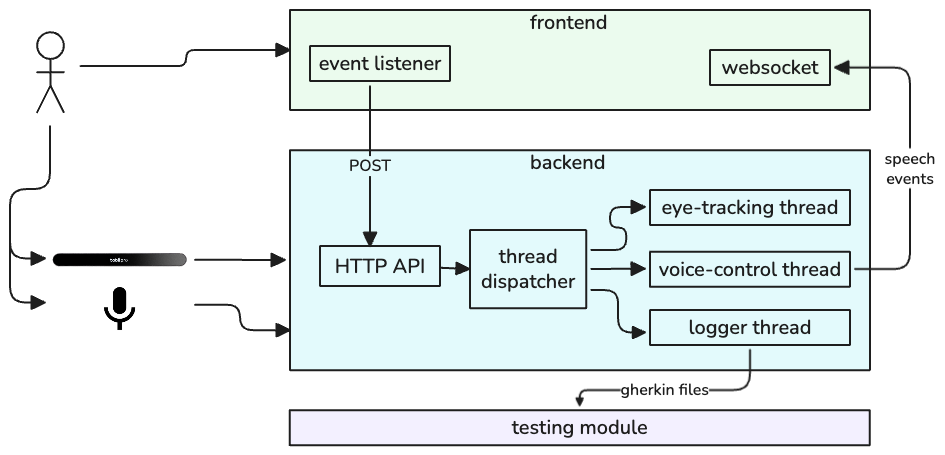
\includegraphics[width=220pt]{imgs/diagram-context.png}
	\caption{Context diagram of the system.}
	% \vspace{-13pt}
	\label{fig:context}
\end{figure}

This section outlines the EyeNav system based on its workflow, as illustrated in Fig.~\ref{fig:context}. EyeNav is composed of 2 main modules: (i) a Chrome Extension sidebar and (ii) a backend module built in python. The Chrome extension sidebar, which functions as an adjacent webpage alongside the main content, presents the available verbal commands, allows to initiate a interaction session, and shows the interpreted verbal commans in realtime once a session has started (See Fig.~\ref{fig:requirements}). Once a session begins, the system orchestrates multiple components, including voice recognition, eye tracking, and interaction logging.

\begin{figure}[h]
	\centering
	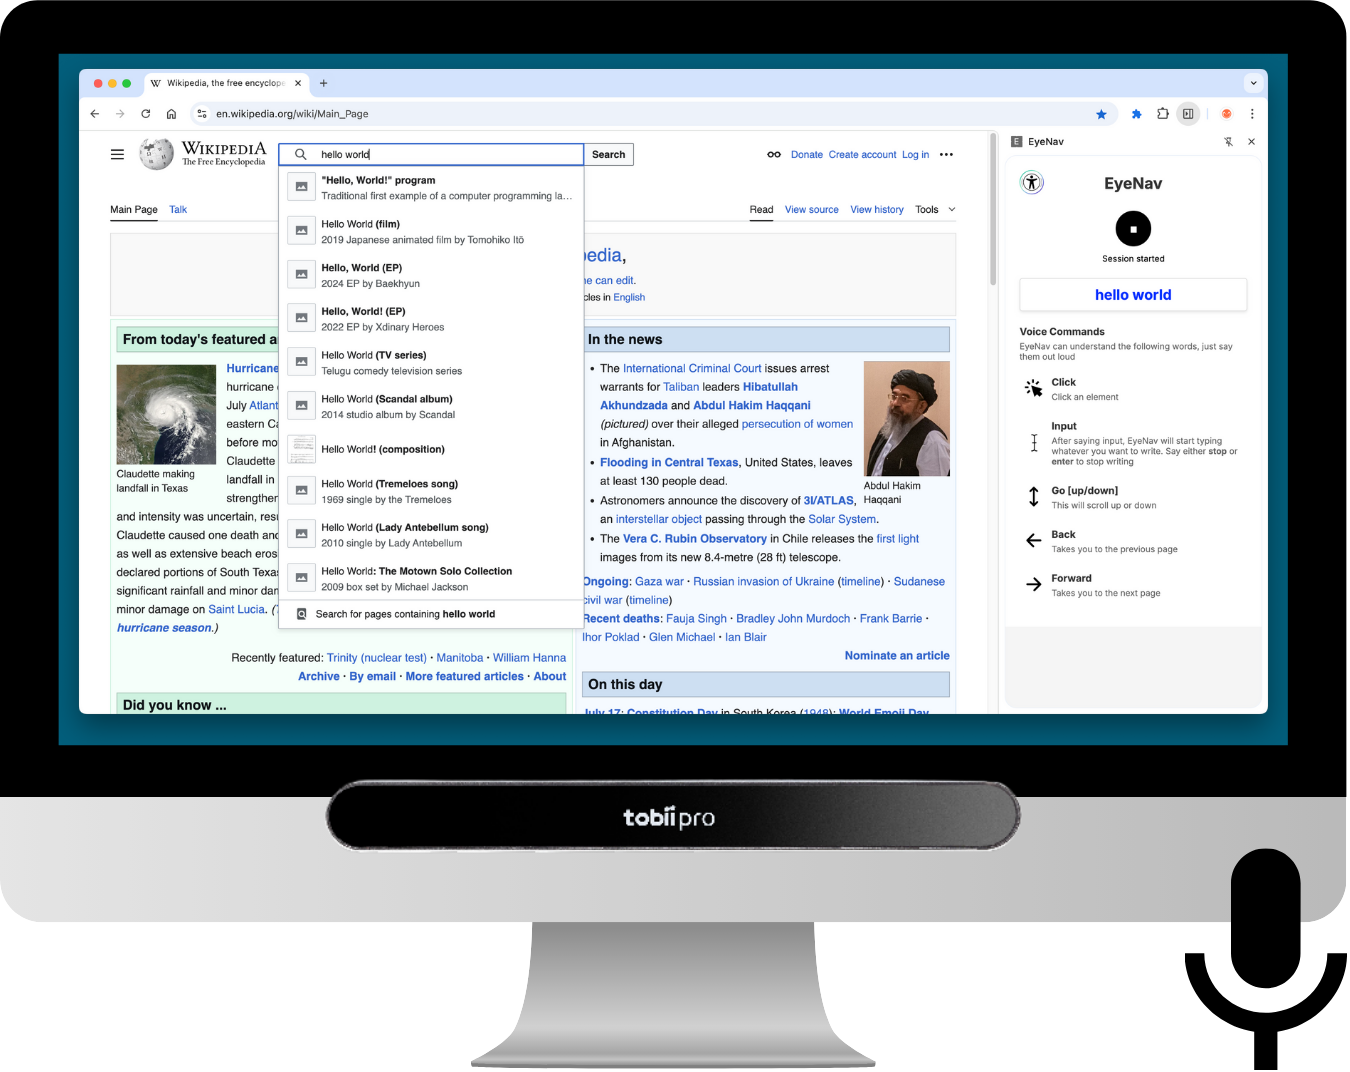
\includegraphics[width=210pt]{imgs/system-requirements.png}
	\caption{A graphic of what the system looks like}
	% \vspace{-13pt}
	\label{fig:requirements}
\end{figure}

User input is captured via an eye tracker and microphone, while the underlying processing occurs in a backend service rather than on the frontend. Concurrently, user interactions, such as clicks, text input, and navigation events, are recorded by a logging module. These recorded events are compiled into an executable test file, which can later be replayed using Gherkin-based test execution tools like Selenium\misref or Kraken\misref.

%\begin{figure}
%    \centering
%    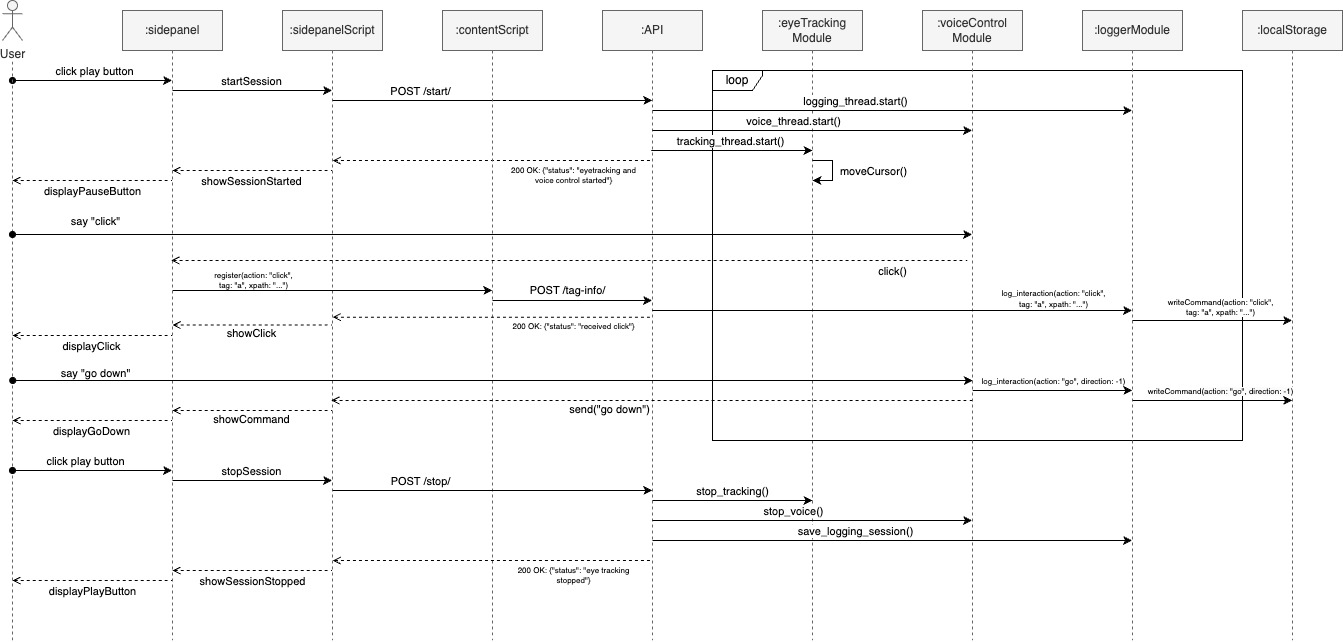
\includegraphics[width=210pt]{imgs/sequence-diagram.jpg}
%    \caption{Sequence diagram. The user starts a session, clicks, scrolls down and then stops the session.}
%    % \vspace{-13pt}
%    \label{fig:sequence-diagram}
%\end{figure}




\subsection{High-Level Architecture}

\begin{figure}
    \centering
    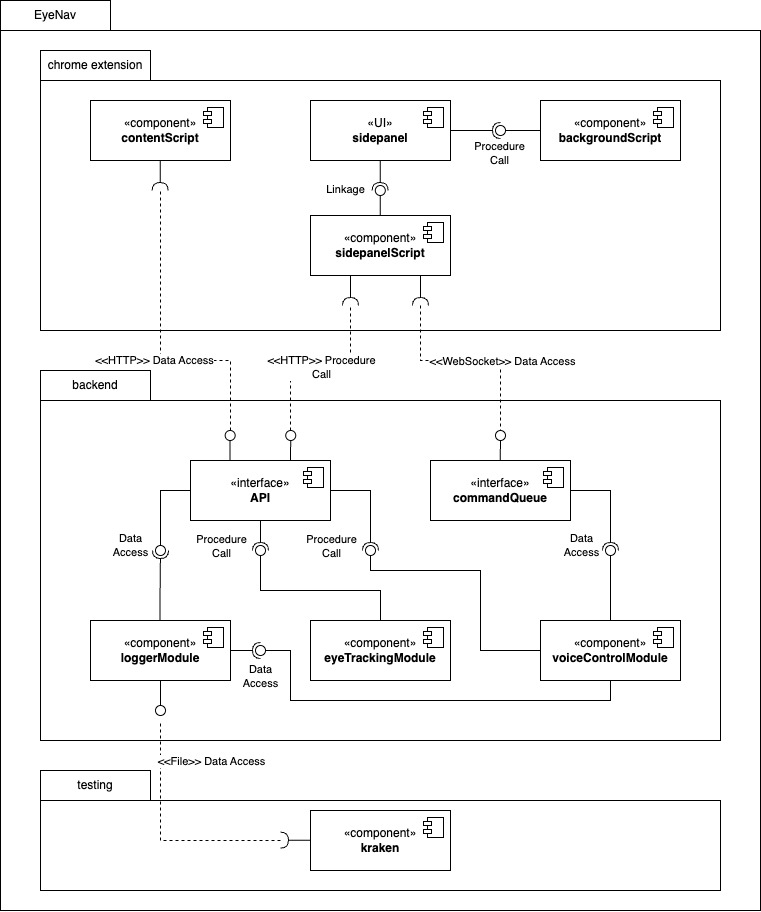
\includegraphics[width=210pt]{imgs/components-diagram.jpg}
    \caption{Components diagram}
    % \vspace{-13pt}
    \label{fig:components-diagram}
\end{figure}

% TODO poner todas las citas de las herramientas

Figure ~\ref{fig:components-diagram} presents the complete component architecture of the system.%, while Figure ~\ref{fig:sequence-diagram} illustrates the system in operation.

The Chrome extension serves as the front-end interface, providing real-time textual feedback for recognized voice commands and capturing user interaction events. Click events are recorded on the frontend and forwarded as HTTP POST requests to the backend to preserve contextual information, such as the associated HTML tag. 

Eye tracking is powered by the Tobii Pro Nano, a single-camera dark/bright pupil system with corneal reflection and a typical latency of approximately 17 ms~\cite{tobiiabndpronano}. The gaze-driven pointer control module uses the \verb|tobii-research| Python SDK to access real-time gaze data and interpolate cursor movement accordingly.

Voice commands are captured through a microphone and transcribed using the Vosk speech recognition engine\misref, which operates entirely on-device for privacy and low latency. Recognized phrases are matched to predefined command templates and sent to the backend over WebSocket connections, enabling minimal response delay.

The backend integrates data from both the Tobii eye tracker and the Vosk engine to interpret user intent, translate inputs into executable UI commands (e.g., clicks, scrolls, text entry), and log all interactions. A dedicated test logging module records each event in Gherkin syntax and compiles reproducible test scripts. These are executed using Kraken, a behavior-driven testing framework built on WebdriverIO\misref, supporting usability and regression testing even under dynamic UI conditions.

The system is organized into modular components, each adhering to a single-responsibility design principle. These include: (1) the gaze-driven pointer control, which enables real-time cursor positioning based on eye movement; (2) the NLP-based command parsing module, which interprets speech input captured by Vosk and maps it to specific UI actions among clicks, text entry, and scrolling; and (3) the record-and-replay test generation module, which logs user interactions in Gherkin syntax and compiles them into executable test scripts compatible with WebdriverIO for automated testing.

\section{EyeNav Capabilities}

\subsection{Voice Commands}

explain briefly the possible commands and how they are interpreted to ensure they are applied (for example, the different ways an element can be identified (id, xpath, ...))

\subsection{NLP in multiple languages}

\subsection{Test Case generation}

Add and example of a generated feature

\subsection{Accessible Interaction (Tab-based and voice-over)}

\section{EyeNev Use Cases}

\CAMILO{Mention the usage case details and the modules that could be "enable" to improve the results, for example for disable users the system does not require test case generation}

\subsection{Accesible Interaction mechanism for web applications}

\subsection{Record and Replay Testing Tool (A-TDD)}

\subsection{Accessibility Experts}

\subsection{Intelligent Agents}

%\section{EyeNav in action}
%
%% \begin{figure}
%%     \centering
%%     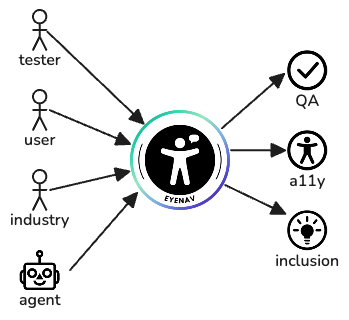
\includegraphics[width=160pt]{imgs/diagram-benefits.png}
%%     \caption{Envisioned users and the possible benefits from using the system}
%%     % \vspace{-13pt}
%%     \label{fig:benefits}
%% \end{figure}
%
%A typical use case starts with the user opening a browser window and launching the Chrome extension side panel. Prior to initialization, the eye tracker is calibrated, and the backend server starts running. When the user hits the start button, the servers starts listening for gaze and voice input, while recording each action in the testing module.
%
%For example: The user gazes at a search bar. $\rightarrow$ Says: “Click.” $\rightarrow$ Says: “Input Nike black shoes.” $\rightarrow$ Says: “Scroll down.” $\rightarrow$ Gazes at a product listing.$\rightarrow$ Says: “Click.”
%
%The recognized commands appear in a side panel for transparency, while the corresponding event interactions are logged by the backend testing module. These logs are stored locally as Gherkin features and step definitions, forming executable test files.


\section{Results}

\subsection{User Feedback}

Qualitative interviews identified several key usability factors. Larger UI elements significantly improved gaze accuracy, making it easier for users to select targets with their eyes. Voice commands were most effective when they were short and distinct, reducing recognition errors. Environmental noise was found to negatively impact the reliability of speech recognition, suggesting the need for robust filtering or alternative input strategies. Users also indicated that visual indicators for "gaze hover targets" would enhance feedback and confidence during interaction. Additionally, simplified scroll commands were perceived as more usable and intuitive compared to earlier, more granular versions.

\subsection{Accessibility Insights}

Testers noted that this input method offers clear benefits for users with limited motor function. However, improvements in UI design (e.g., reachable icons) are needed for full accessibility compliance. Due to scope limitations, no participants with motor impairments were included, though future studies aim to address this.

% the design of planned studies (for early prototypes)

\section{Discussion}

The integration of eye-tracking and NLP proved effective for hands-free interaction in a browser context. Further work is needed to improve performance in varied environments (e.g., low-light, users with glasses, non-native accents). Eye-based clicking was responsive but may require calibration for precision.

The testing module provided reproducible, human-readable test cases for interaction flows. While brittle on dynamic pages, these cases proved valuable for visual regression or task analysis. 

This architecture design allows for the combination of many of the purposes eye-tracking has already; we can analyze user behavior, identify usability bottlenecks, and validate system performance under varying conditions. This is especially valuable in eye-tracking based systems, where subtle differences in gaze patterns can significantly influence interaction outcomes. Replay tools also facilitate comparative evaluations, allowing different interface versions or input modalities to be tested using identical interaction sessions.

% \subsection{Planned Studies}
% TODO

\section{Future Work}

Planned improvements include enhancing support for users who wear glasses through prescription lens calibration techniques, and extending system compatibility to mobile and AR/VR platforms. Additional enhancements involve creating onboarding guides and integrating visual cues to facilitate learning gaze-based input, as well as including individuals with motor impairments in future user studies to better validate accessibility benefits. The system's test recorder is also being developed as a standalone tool to support broader usability testing efforts. Finally, there are plans to explore integration with immersive environments, such as the Apple Vision Pro and Meta Quest, to evaluate usability and responsiveness in mixed-reality contexts.

% !TEX root = main.tex

\section{Conclusion \& Future Work}
%    - Summarize main contributions: novel tool, accessibility impact, testing automation.
%    - Emphasize readiness for live demo and replicability (public code/datasets).
% TODO
a



\balance
\bibliographystyle{IEEEtran}
\bibliography{local,bib/testing,bib/tools}

\end{document}
